\documentclass[a4paper,twoside,kulak]{kulakreport}
% LATEX CLASSES
% Standaard: article, report, book, beamer, sciposter
% Huisstijl: kulakarticle, kulakreport, kulakbook, kulakbeamer, kulaksciposter

% PREAMBULE
% dit is het gedeelte tussen \documentclass en de \begin{document}
% hier worden extra pakketten geladen en instellingen gemaakt

% Essentiële pakketten aan het begin van de preambule om correct compileren mogelijk te maken
\usepackage[utf8]{inputenc} % Correct vreemde symbolen inlezen
\usepackage[dutch]{babel}   % Nederlandstalige regels voor woordafbreking
\usepackage[T1]{fontenc}    % Correct vreemde symbolen weergeven
\usepackage{float}

% Instellingen voor titelpagina, kop- en voettekst
% In een standaard article-document zijn er minder mogelijkheden
\faculty{Wetenschap \& Technologie Kulak}
\group{}
\title{Human Pose Estimation:\\Toepassing}
\subtitle{}
\author{Isaac venus\\Stan Vanhecke\\Mathieu Vanooteghem}
% \\Stan Vanhecke\\Mathieu Vanooteghem
\emailaddress{isaac.venus@student.kuleuven.be}
% \\stan.vanhecke@student.kuleuven.be\\mathieu.vanooteghem@student.kuleuven.be
\institute{KU Leuven Kulak, Wetenschap \& Technologie}
\date{Titularis: Koen Van Den Abeele\\Begleider: Jens Goemare\\Academiejaar 2020 -- 2021}
\address{
   KU Leuven Kulak           \\
   Wetenschap \& Technologie \\
   Etienne Sabbelaan 53, 8500 Kortrijk             \\
   Tel.\ +32 56 24 60 20     \\
   \href{mailto:\theemailaddress}{\texttt{\theemailaddress}}
   }

\begin{document} % hier begint de eigenlijke inhoud van het document

\titlepage

\tableofcontents

\chapter*{Inleiding}
Aan materiaal in de medische wereld hangt steeds een stevig prijskaartje, dus vroegen wij ons af hoe we dit wat vriendelijker kunnen maken voor de portefeuille. Wat natuurlijk niet mag is het gebruik van hoogtechnologische medishe apparatuur maar dat er in de plaats de technologie gebruikt wordt die iedereen al heeft zoals een laptop en een smartphone. We moeten dus software schrijven die met de elektrica die we al hebben kan werken. In dit verslag richten wij ons op \emph{human pose estimation} (HPE), of lichaamspositiebepaling. We gebruiken hiervoor de open-source HPE software openpose die via neurale netwerken de positie van een persoon schat op een foto. Met dit programma kunnen we dan software schrijven voor medische doeleinden.

\chapter{HPE, revolutionair?}
HPE is gemakkelijk, snel, goedkoop en steeds nauwkeuriger
heatmaps en kansen uitleg en over openpose specifiek
vermelden dat het werkt met neurale netwerken (cfr. infra)

\chapter{Theoretische achtergrond}
\section{Openpose}
Openpose is een open-source 
\section{Neurale netwerken}

Een (artificieel) neuraal netwerk of ANN is een netwerk geïnspireerd op een biologisch neuraal netwerk zoals die voorkomt in hersenen met de bedoeling om deze iets te doen leren. Het ANN is opgebouwd uit artificiële neuronen die een neuron in een brein moeten voorstellen. Al de neuronen zijn verbonden met andere neuronen en kunnen signalen uitsturen en ontvangen. In een ANN zijn de signalen getallen en kan elk neuron een bepaalde bewerking uitvoeren op een binnenkomend signaal om deze verder te sturen. Elke connectie heeft ook een gewicht dat bepaalt hoe sterk het signaal is dat hij uitstuurt. Dit gewicht past zich aan als het neuraal netwerk leert. 

\subsection{Opbouw van een neuraal netwerk}
\paragraph{Neuronen}
Zoals er hierboven staat is een artificieel neuron geïnspireerd op een neuron uit een brein. Elk neuron heeft een of meerdere inputs en één output die kan verzonden worden naar meerdere andere neuronen. De input van een neuron kan ofwel komen van de data die in het neuraal netwerk wordt gestoken of van andere neuronen. De output van de \emph{output neurons} is wat uit het programma komt. Om de output van een neuron te berekenen neem je de gewogen som van de inputs, met als gewicht de waarden van de connecties. Er wordt ook nog een bias opgeteld bij de output.

\paragraph{Connecties}
Om te kunnen leren moet de data natuurlijk kunnen worden doorgegeven van het ene neuron naar de andere. Dit verloopt via een “connectie” die een bepaald gewicht heeft dat de sterkte en daarmee ook het belang van een bepaalde connectie weergeeft.

\paragraph{Lagen}
Een neuraal netwerk bestaat uit meerdere lagen van neuronen, meer bepaald de \emph{input layer}, \emph{hidden layers} en \emph{output layer} \ref{netwerk}. Zoals de namen wel duidelijk maken geef je de data aan de \emph{input layer} en komen de berekende waarden uit de \emph{ouput layer}. Daartussen zijn er eventueel \emph{hidden layers}. Tussen twee lagen zijn er meerdere manieren van connecties tussen de neuronen mogelijk.

\begin{figure}
	\begin{center}
		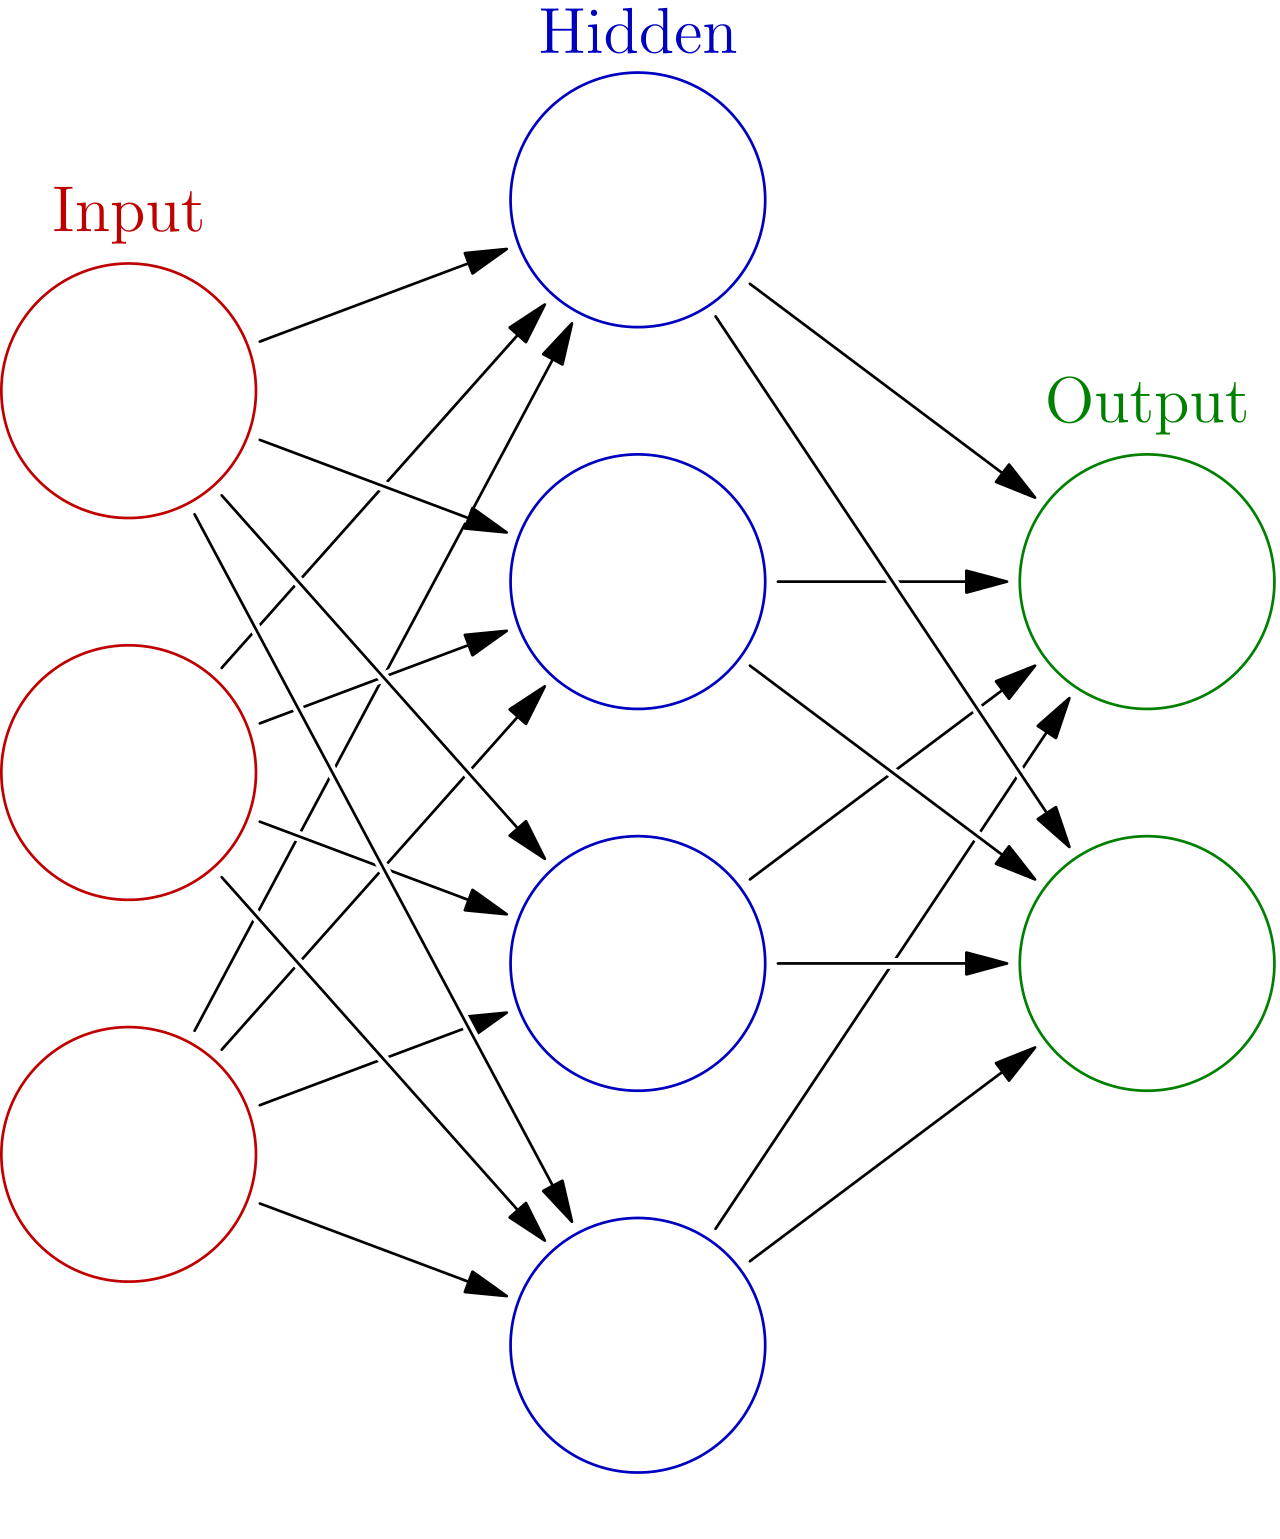
\includegraphics[width=8cm]{netwerk.png}
	\end{center}
	\caption{Voorbeeld van een neuraal netwerk. (afbeelding van wikipedia.org)}
	\label{netwerk}
\end{figure}

\subsection{Trainen van een neuraal netwerk}
Bij het programmeren van een neuraal netwerk weet je natuurlijk niet wat de gewichten zijn van alle connecties. Je moet het model dus doen leren. Dit doe je door de gewichten (over meerdere leercycli) aan te passen zodat de output zo goed mogelijk past bij het gewenste resultaat. Er zal altijd een bepaalde fout op de output zitten dus het model gaat nooit perfect zijn. Het trainen van een model is gedaan als de fout op de output niet meer verkleint en dus een minimum heeft bereikt. Het aanpassen van de gewichten gebeurt met een zekere \emph{learning rate}. Dit bepaalt de grootte van de correcties die gebeuren bij de gewichten. Bij een grote \emph{learning rate} kan je model snel gedaan zijn met leren maar meer kans op een grotere fout op de output. Een kleine \emph{learning rate} zal het trainen vertragen maar je uiteindelijke resultaat zal beter zijn.



\chapter{Toepassingen}
Zoals eerder al gezegd zullen we ons focussen op toepassingen in de medische wereld dat gebruik kan maken van HPE waarvoor wij een goedkope oplossing kunnen ontwikkelen. Hierbij testen we mogelijke problemen en analyseren we of dit wel een goede optie is. We proberen dit dan allemaal op een methodische manier uit te werken, waarbij we een specifiek geval steeds breder gaan bekijken.


Een eerste toepassing is het opvolgen van de revalidatie na een schouderoperatie. Met een foto gemaakt met een gsm kunnen wij een analyse uitvoeren van de beweging van de schouder na de operatie.

Een tweede en uitgebreidere toepassing is het analyseren van de positie op de fiets. Veel amateurwielrenners hebben een slechte houding op de fiets en een professionele bikefitting kost al snel een paar honderd euro. Via lichaamspositiebepaling kunnen wij weer met een simpele foto de positie bepalen op de fiets en dan correcties voorstellen. Dit is een goedkope oplossing die voor een zeer breed publiek inzetbaar is. Voor professionele wielrenners zal dit wel waarschijnlijk niet voldoende zijn, maar voor een amateur kan dit een goedkoop alternatief zijn.



\section{Toepassing 1: opvolgen van revalidatie na schouderoperatie}
\subsection{Bepalen van de hoek tussen arm en lichaam}

We willen meten hoe ver een persoon zijn arm kan roteren voor de opvolging van de revalidatie na een schouderoperatie. Hiervoor kunnen we de hoek tussen het opperarmbeen en een ander lichaamsdeel bepalen. Op figuur \ref{fig:skelet} komt dat dus neer op de hoek bepalen van de lijnstukken [32] en [21] of [65] met een ander lichaamsdeel. Als we Openpose gebruiken om de positie te schatten van een persoon op een foto krijgen we als output de coördinaten van de verschillende knooppunten. Met deze coördinaten hebben we voldoende informatie om de hoek te berkenen en zo objectieve informatie te krijgen over het verloop van de revalidatie.


Bij een foto vanuit vooraanzicht kunnen we berekenen hoe ver de patiënt zijn arm zijwaarts omhoog kan brengen. Bij een foto genomen vanuit zijaanzicht kunnen we berekenen hoe ver hij de arm vooruit kan omhoog steken. Het is we belangrijk dat de foto altijd vanuit dezelfde positie wordt getrokken omdat er anders variatie kan zijn op de hoek.



\begin{figure}[H]
	\centering
	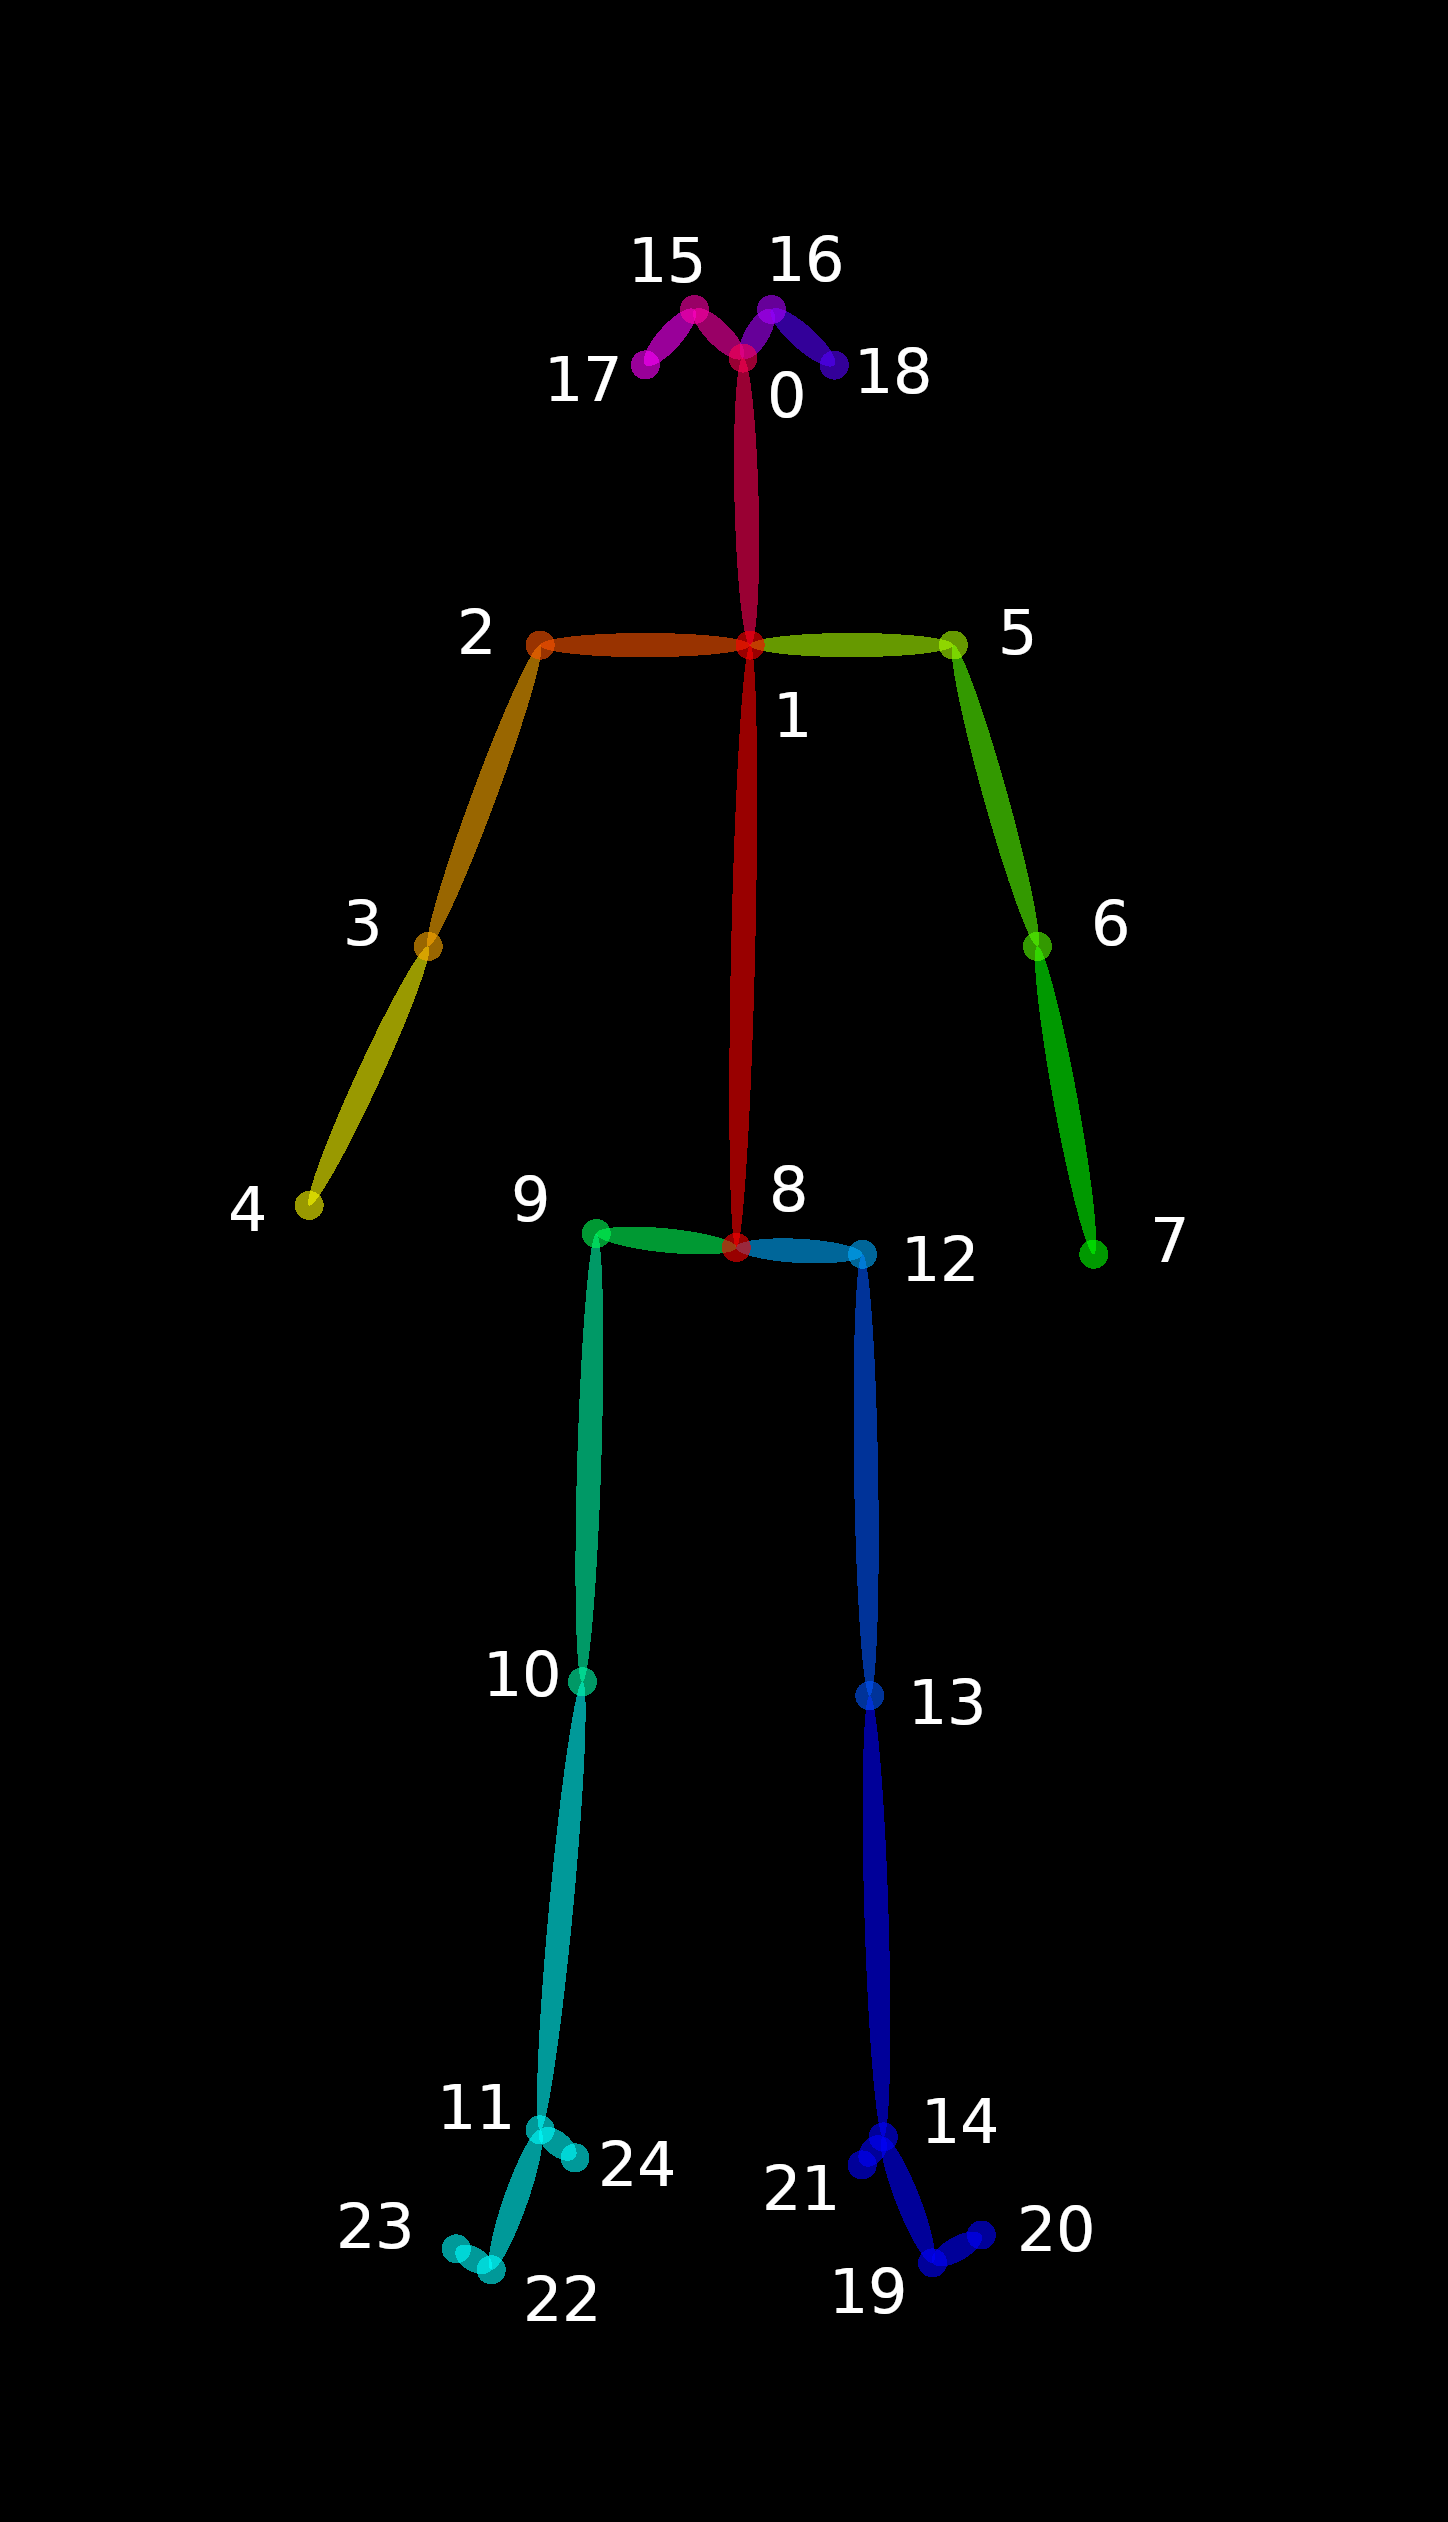
\includegraphics[width=.5\textwidth]{HPE_skelet}
	\caption{Voorstelling van de positie bepaald via Openpose (afbeelding van \href{https://github.com/CMU-Perceptual-Computing-Lab/openpose/blob/master/doc/output.md}{openpose})}
	\label{fig:skelet}
\end{figure}


\subsection{Voorlopige resultaten}

Via Openpose krijgen we de coördinaten van alle punten die openpose kan herkennen. Hiermee kunnen we dan verder onderzoek doen. Op dit moment zijn we in staat om hoeken tussen bepaalde lichaamsdelen te berekenen met als doel objectieve gegevens te bekomen tijdens bijvoorbeeld een revalidatie na een ongeval.

\paragraph{Wiskundige achtergrond}
Om de hoek tussen twee lichaamsdelen te berekenen gebruiken we de cosinusregel. Hier volgt een klein beetje duiding over hoe we die precies gebruiken (zie figuur \ref{cos}).\\

\begin{figure}[H]
	\begin{center}
		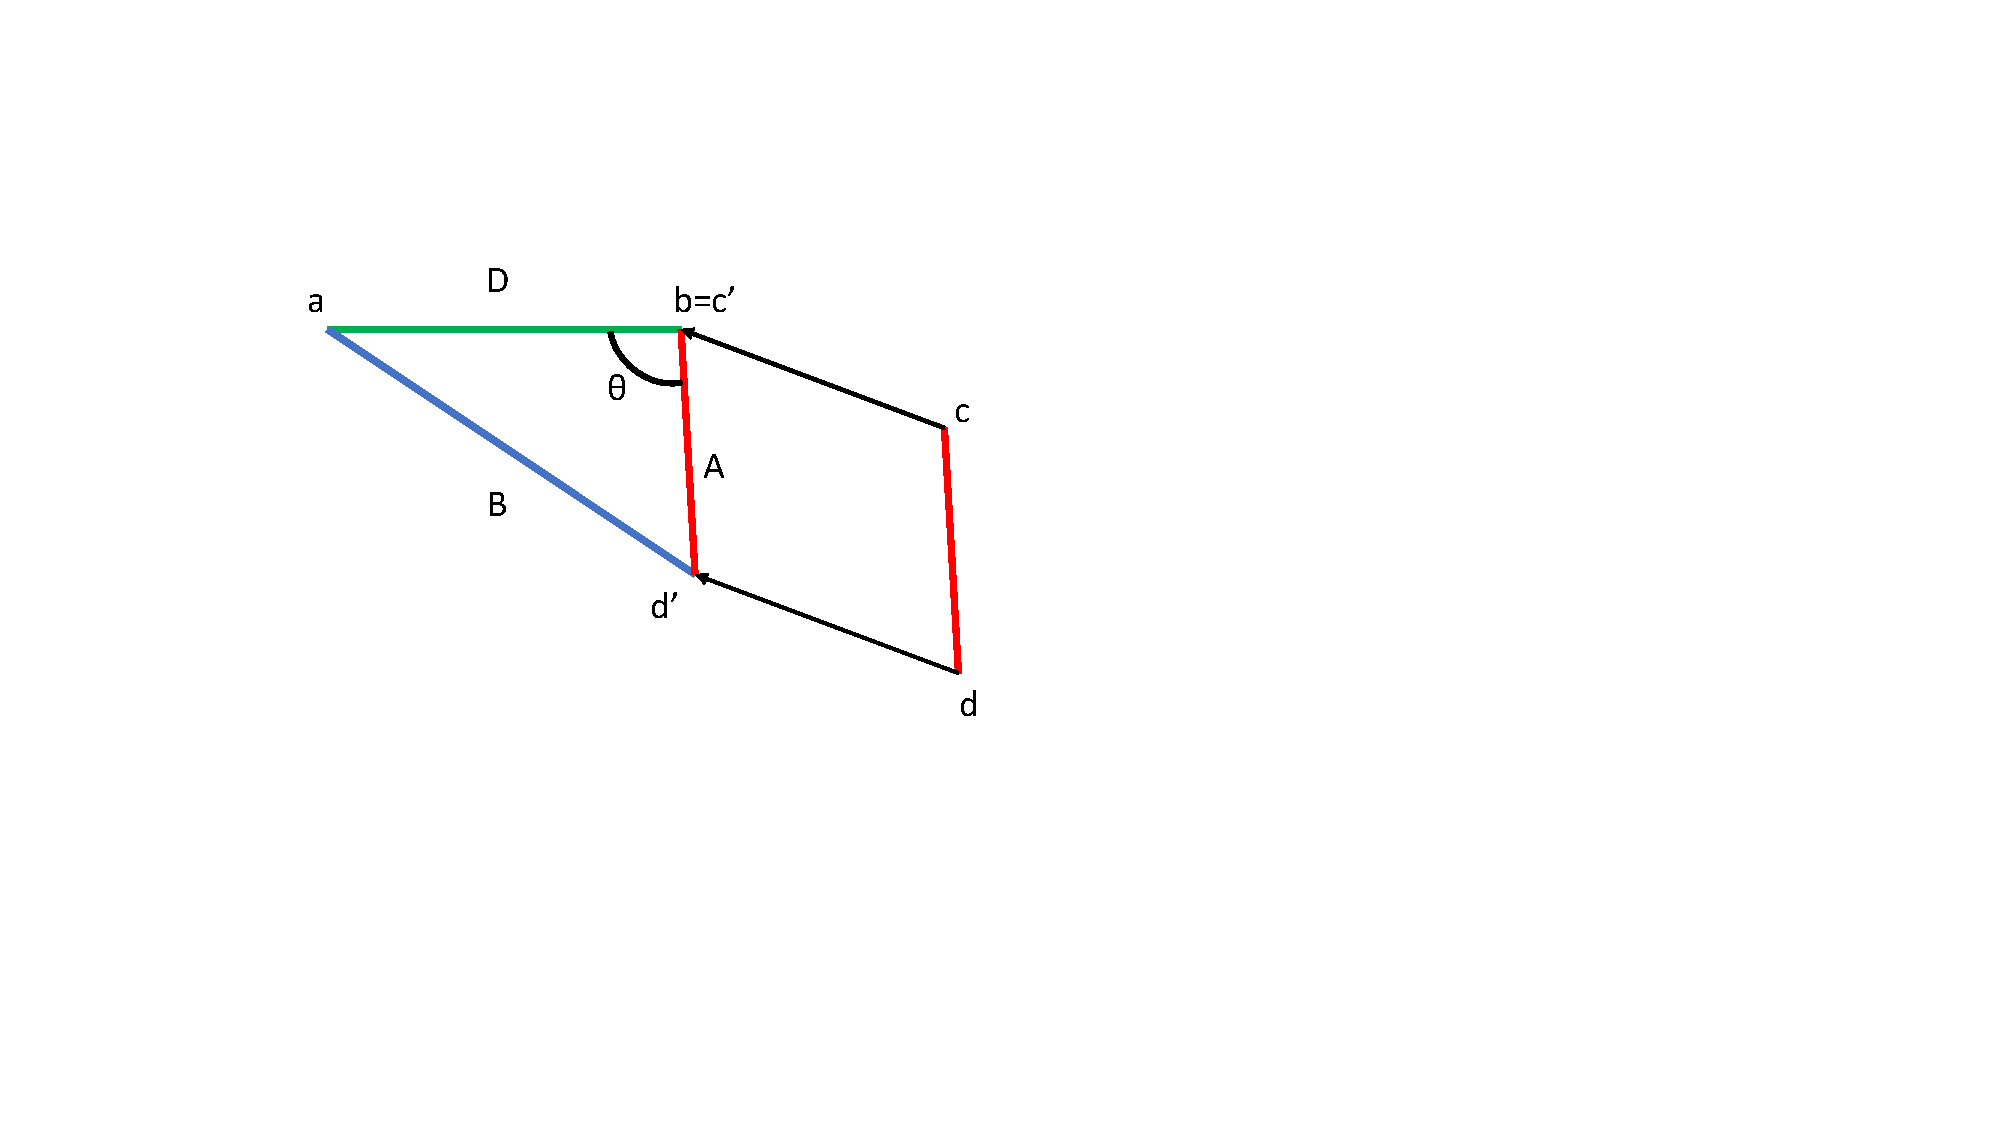
\includegraphics[width=10cm]{cos.pdf}
	\end{center}
	\caption{Hoek tussen 2 lichaamsdelen}
	\label{cos}
\end{figure}

We stellen \(a, b\) de coördinaten die het eerste lichaamsdeel afbakenen en \(c, d\) de coördinaten van het tweede lichaamsdeel. De hoek tussen de lichaamsdelen is dan de \(\theta\) van op de figuur. We kunnen gewoon de cosinusregel gebruiken om de hoek te bepalen als we \(c\) op \(b\) leggen. We krijgen dan
\[B^2 = A^2 + D^2 -2\cdot A\cdot D\cos\theta\]
en dus
\[\cos\theta = \frac{A^2 + B^2 - B^2}{2\cdot A\cdot D}\]
met
\[A = \sqrt{(d_x - c_x)^2 + (d_y - c_y)^2}\]
\[B = \sqrt{(b_x - a_x + d_x - c_x)^2 + (b_y - a_y + d_y - c_y)^2}\]
\[D = \sqrt{(b_x - a_x)^2 + (b_y - a_y)^2}\]
Als we dus de 4 coördinaten weten kunnen we de hoek bepalen.
\paragraph{Voorbeeld}
Een voorbeeld bij het bepalen van een hoek tussen is afbeelding \ref{samen}. Als we de hoek bereken tussen de ruggengraat (rood) en het opperarmbeen(licht oranje) krijgen we als waarde:
\begin{itemize}
	\item 1: 21.63 graden
	\item 2: 78.06 graden
	\item 3 130.00 graden
\end{itemize}
\begin{figure}
	\begin{center}
		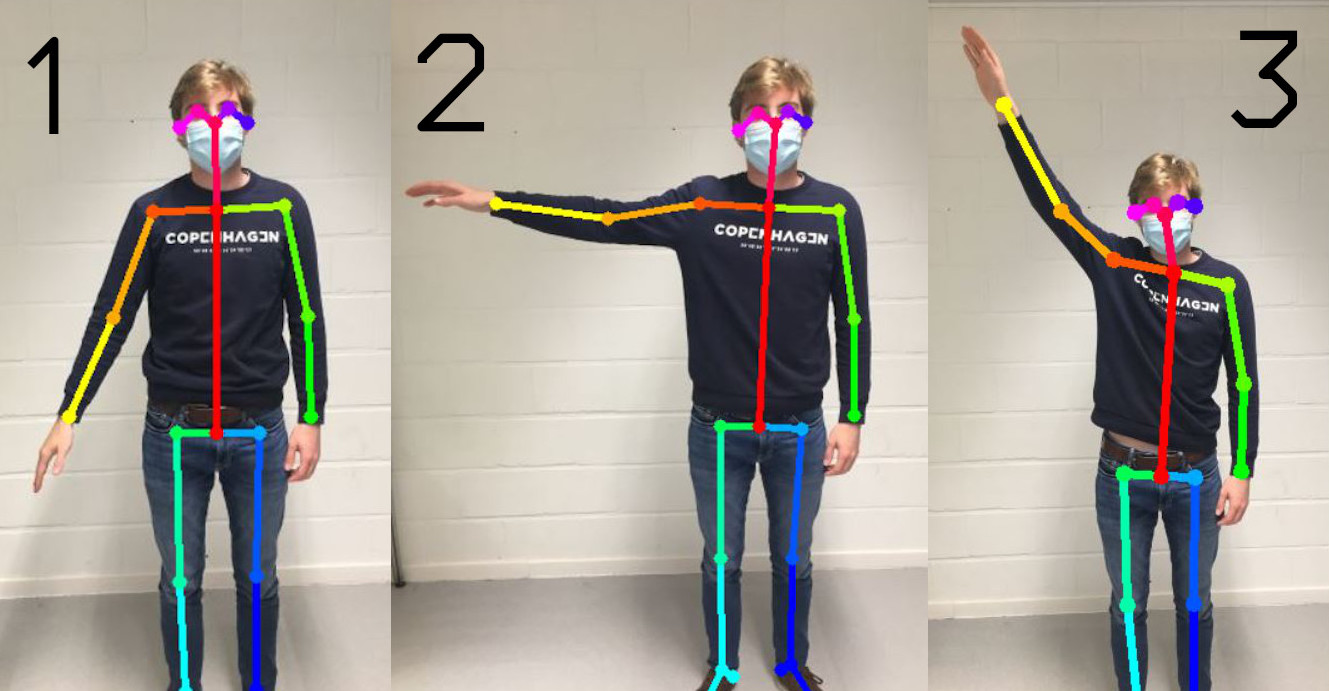
\includegraphics[width=12cm]{samen.jpg}
	\end{center}
	\caption{Voorbeeld bij het bepalen van een hoek.}
	\label{samen}
\end{figure}
\subsection{Voorlopige conclusies}
Door deze  toepassing weten we dat het relatief eenvoudig is om met openpose zinvolle berekeningen te kunnen doen. Door de coördinaten die gegeven worden als output kunnen we gemakkelijk programma's schrijven die hiermee werken.


\section{Toepassing 2: fietspositie bepalen}
Voor de tweede toepassing willen we een goedkoper alternatief bieden voor een bikefitting. Hierbij worden er foto's getrokken van de persoon op de fiets en kunnen we dan op basis van de positie bepaald met openpose eventuele correcties uitvoeren op de fiets.

\begin{figure}[H]
	\centering
	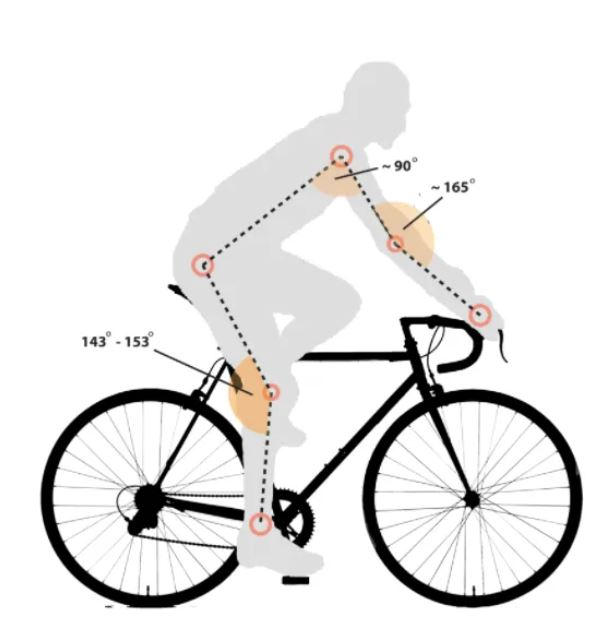
\includegraphics[width=\textwidth]{bikefit}
	\caption{Verschillende hoeken voor optimale positie op de fiets}
	\label{fig:bikefit}
\end{figure}

\begin{figure}[H]
	\centering
	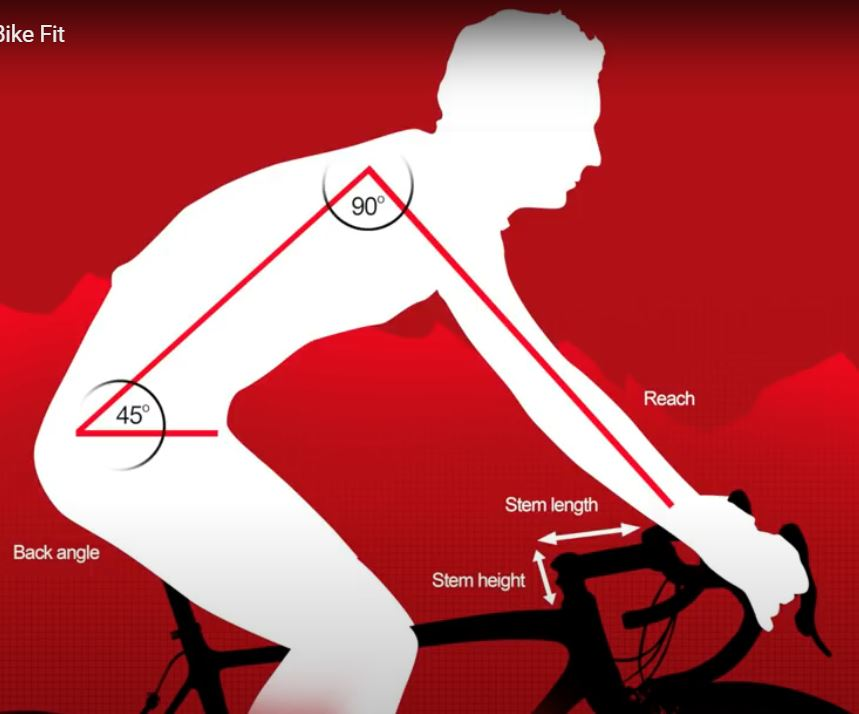
\includegraphics[width=\textwidth]{bikefit_romp}
	\caption{Optimale hoek die het bovenlichaam maakt met de horizontale}
	\label{fig:bikefit_romp}
\end{figure}

\subsection{Voorlopige resultaten}
Komt op finaal verslag.

\subsection{Voorlopige conclusies}
Komt op finaal verslag.

\chapter{Vakintegratie}
Het is natuurlijk belangrijk om dit project een plaats te geven binnen onze opleiding ingenieurswetenschappen. We bekijken welke vakken uit de eerste 3 semesters van onze bachelor het meest gebruikt worden tijdens dit project. De belangrijkste link is met het vak begingselen van programmeren. In dit vak leerden we werken met Python en verworven we inzicht in het programmeren. Wat heel handig is, want tijdens ons project maken we veelvuldig gebruik van Python. Elk zelf gemaakt programma is geschreven in Python want Openpose heeft een uitstekende Python API. Verder maakt wiskunde ook een groot deel uit van ons project, want het berekenen van hoeken of afstanden kan niet zonder de wiskunde. We gebruiken hierbij kennis uit verschillende wiskundige vakken zoals, Analyse \& calclus en Lineaire algebra. Als laatste kunnen we Statistiek ook nog linken aan dit project aangezien Openpose enkel een schatting geeft van de lichaamspositie. Het werkt met \textit{heatmaps} en kiest per knooppunt dan het coördinaat met de hoogste kans. We gebruiken zelf geen statistische technieken, het helpt ons wel bij het begrijpen van Openpose.

\chapter{Planning}
(gantt chart enzo\texttt{})

\chapter*{Referenties}
\bibliographystyle{plainnat}
\bibliography{biblio}
\printindex

\end{document}